\chapter{Kajian Pustaka}
Tugas akhir ini membahas perancangan sistem pengawasan jantung. Untuk mendirikan landasan berfikir, bab ini akan membahas teori dan fakta yang berkaitan dengan perancangan sistem tersebut.

\section{ECG dan PPG}
Terdapat 2 jenis sensor yang umum digunakan untuk melakukan \textit{monitoring} jantung, yaitu \textit{Electrocardiogram} (ECG) dan \textit{Photoplethysmogram} (PPG) seperti yang terlihat pada gambar \ref{fig:ecg_n_ppg}. Kedua jenis sensor ini menjadi pilihan utama dalam \textit{monitoring} jantung karena keduanya mengusung konsep \textit{non-invasive}. Sensor non-invasive memungkinkan melakukan pengambilan data tubuh tanpa perlu melukai/menusuk bagian tubuh tertentu. Secara umum ECG akan menghasilkan pengukuran lebih akurat dari pada PPG. Namun PPG lebih nyaman digunakan dalam jangka panjang dari pada ECG.

\begin{figure}[h!]
    \centering
    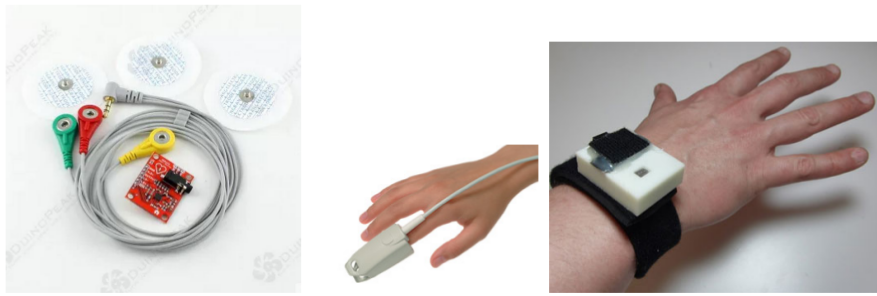
\includegraphics[scale=0.3]{images/sensors.png}
    \caption{a. Sensor ECG dengan 3 titik timbal; b. Sensor PPG ujung jari; c. Sensor PPG di pergelangan tangan}
    \label{fig:ecg_n_ppg}
\end{figure}

\subsection{Titik Fiducial}
Sebuah siklus sinyal ECG dapat dilihat menjadi beberapa titik \textit{fiducial} (pembanding) yaitu P-QRS-T, seperti terlihat pada gambar \ref{fig:ecg_points}. Sedangkan siklus sinyal PPG dilihat menjadi siklus Diastolic-Systolic-Dicrotic seperti terlihat pada gambar \ref{fig:ppg_points}

\begin{figure}[h!]
    \centering
    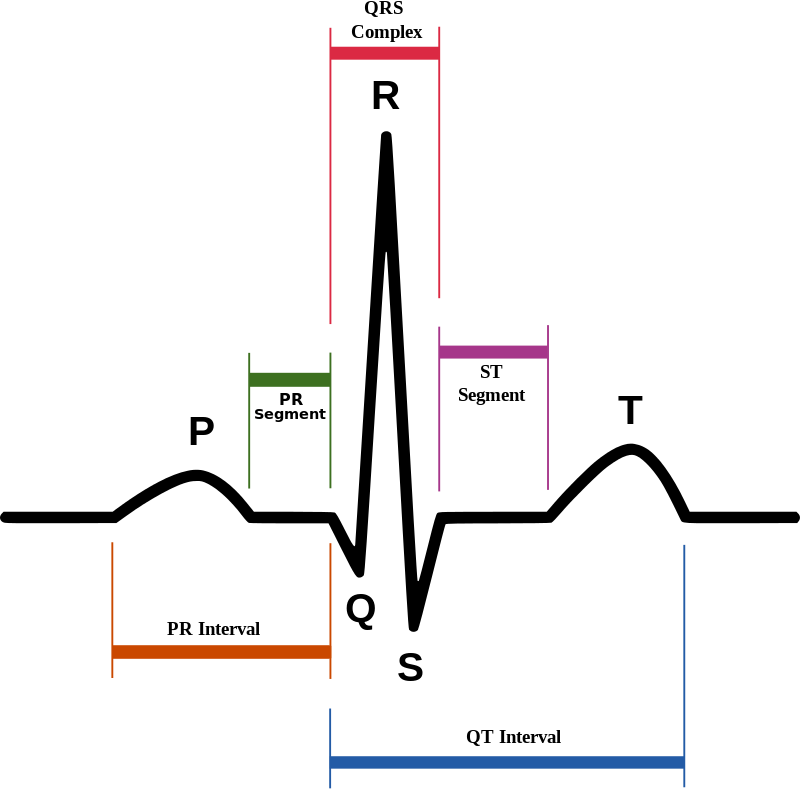
\includegraphics[scale=0.2]{images/ecg_points.png}
    \caption{Sinyal ECG berdasarkan titik fiducial}
    \label{fig:ecg_points}
	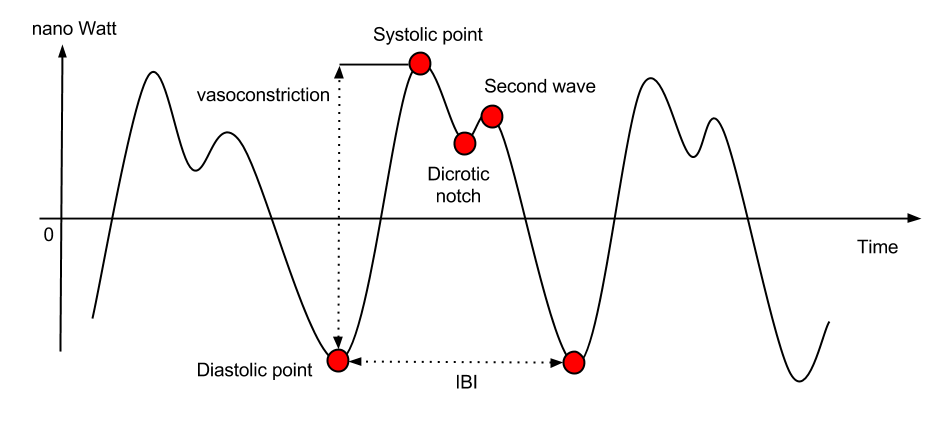
\includegraphics[scale=0.3]{images/PPG2.png}
    \caption{Sinyal PPG berdasarkan titik fiducial}
    \label{fig:ppg_points}
\end{figure}


\subsection{Pembacaan Sinyal}
Walaupun kedua jenis sensor dapat digunakan untuk monitor jantung, sinyal yang dihasilkan sedikit berbeda, terlihat pada gambar \ref{fig:ecg_vs_ppg} \cite{ppg_vs_ecg}. Secara langsung dapat dilihat sinyal hasil dari PPG dengan ECG berbeda secara morfologi (bentuk). Karena sumber sinyal yang sama (dari jantung) siklus PPG dan ECG dapat disinkronisasi (saling dipetakan) berdasarkan titik R pada ECG dan puncak sistolik pada PPG seperti gambar \ref{fig:ecg_vs_ppg2} \cite{ecg_syncro}. Perbedaan waktu kemunculan R dan Sistolik dikenal sebagai \textit{Pulse Arrival Time} (PAT). PAT dapat digunakan sebagai parameter mengukur tekanan darah, yang mana tidak dicakup pada tugas akhir ini.

\begin{figure}[H]
    \centering
    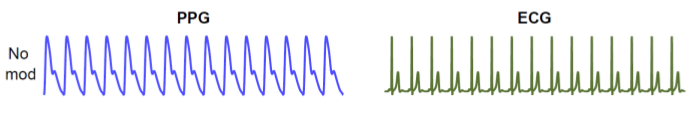
\includegraphics[scale=0.6]{images/ecg_vs_ppg.png}
    \caption{Perbandingan sinyal ideal PPG dan ECG}
    \label{fig:ecg_vs_ppg}
	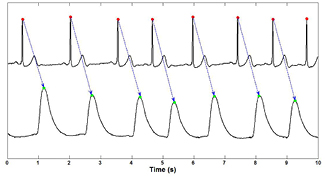
\includegraphics[scale=0.8]{images/sinkronisasi.jpg}
    \caption{Sinkronisasi antara ECG dan PPG}
    \label{fig:ecg_vs_ppg2}
\end{figure}

\section{Aritmia}
Aritmia adalah kategori gangguan jantung yang berupa irama jantung yang tidak normal. Beberapa panyakit jantung yang tergolong aritmia ialah \textit{Tachycardia} (detak lebih cepat dari normal), \textit{Bradycardia} (detak lebih lambat dari normal), \textit{Premature Atrial Contraction} (PAC), \textit{Premature Vantricular Contraction} (PVC), \textit{Ventricular Tachycardia} (VT), dan \textit{Ventricular Fibrillation} (VF). Contoh kemunculan PAC, PVC dan VF dapat dilihat pada gambar \ref{fig:contoh_aritmia}.

\begin{figure}[H]
    \centering
	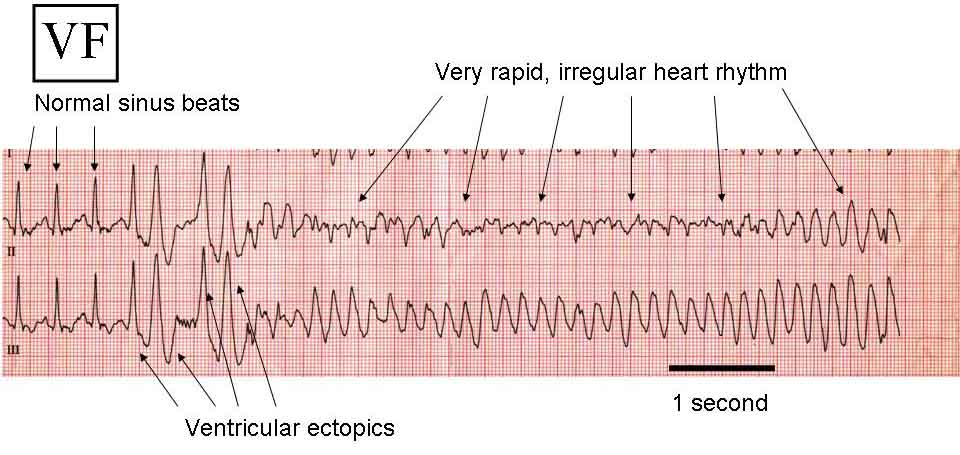
\includegraphics[scale=1.2]{images/VF.jpg}
    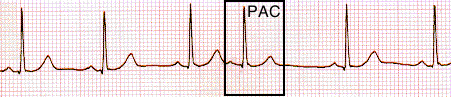
\includegraphics[scale=0.5]{images/PAC1.png}
	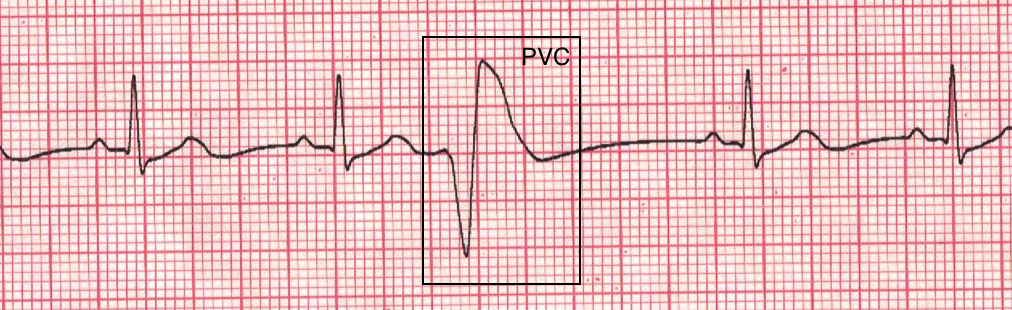
\includegraphics[scale=0.25]{images/PVC1.png}
    \caption{a. Sinyal VF; b. Sinyal PAC; c. Sinyal PVC}
    \label{fig:contoh_aritmia}
\end{figure}

\subsection{Riset Klasifikasi Aritmia Otomatis}
Untuk mengklasifikasian aritmia seorang dokter perlu melihat hasil rekam jantung seorang pasien baik rekam ECG maupun PPG. Akan sangat melelahkan jika seorang dokter secara terus menerus memeriksa rekam jantung seorang pasien. Oleh karena itu dibutuhkan sebuah algoritma yang dapat melakukan klasifikasi secara otomatis. 

Telah banyak penelitian yang dilakukan untuk melakukan otomasi klasifikasi aritmia[xx]. Kini penelitian tersebut telah memiliki keakuratan yang cukup baik, mencapai 90\%, dengan berbagai macam metode dan ekstraksi fitur.

Pada tahun xxx, asme asme asem

Pada tahun xxx, asme asme asem

Pada tahun xxx, asme asme asem

Pada tahun xxx, asme asme asem

Pada tahun xxx, asme asme asem

Pada tahun xxx, asme asme asem

\begin{table}[H]
\centering
	\begin{tabular}{|c|c|c|c|c|}
	\hline
	\rowcolor{gray}
	\textbf{Judul} & \textbf{Penulis} & \textbf{Fitur} & \textbf{Metode}  & \textbf{Hasil}\\
	\cline{1-5}
	Penemuan bla bla adu adu & Alif Akbar & Titik R & Decisin & 90\% \\
	\cline{1-5}
	Penemuan bla bla adu adu & Alif Akbar & Titik R & Decisin & 90\% \\
	\cline{1-5}
	Penemuan bla bla adu adu & Alif Akbar & Titik R & Decisin & 90\% \\
	\hline
	\end{tabular}
	\caption{Street Data}
	\label{table:tbljalan}
\end{table}

\section{Produk Monitoring Jantung di Pasaran}
Meningkatnya kesadaran masyarakat akan penyakit jantung mendorong banyak perusahaan untuk membuat produk \textit{monitoring} jantung. Perusahaan seakan berlomba memproduksi alat monitoring baik yang berstandar medis untuk penggunaan rawat intesif maupun yang tidak berstandar medis untuk penggunaan sehari hari. Salah satu perusahaan yang ikut memproduksi alat \textit{monitoring} ialah perusahaan raksasa dari Korea, Samsung, yang mengeluarkan "Gear S3" pada tahun 2017 []. Selain produk berbentuk alat (\textit{hardware}), produk berbentuk program (\textit{software}) yang hanya memanfaatkan \textit{flash} di kamera \textit{smartphone} sebagai sensor PPG juga banyak ditemukan[xx-xx-xx].

\begin{figure}[H]
    \centering
	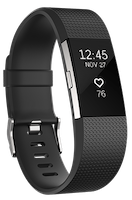
\includegraphics[scale=0.4]{images/fitbit.png}
    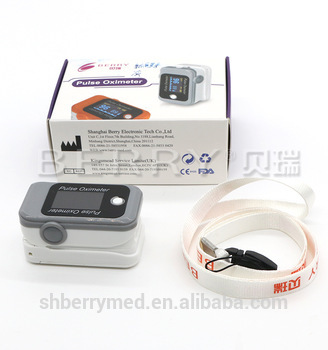
\includegraphics[scale=1]{images/ppg_clip.jpg}
	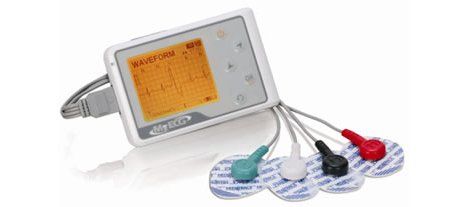
\includegraphics[scale=0.3]{images/ecg_1.jpg}	
	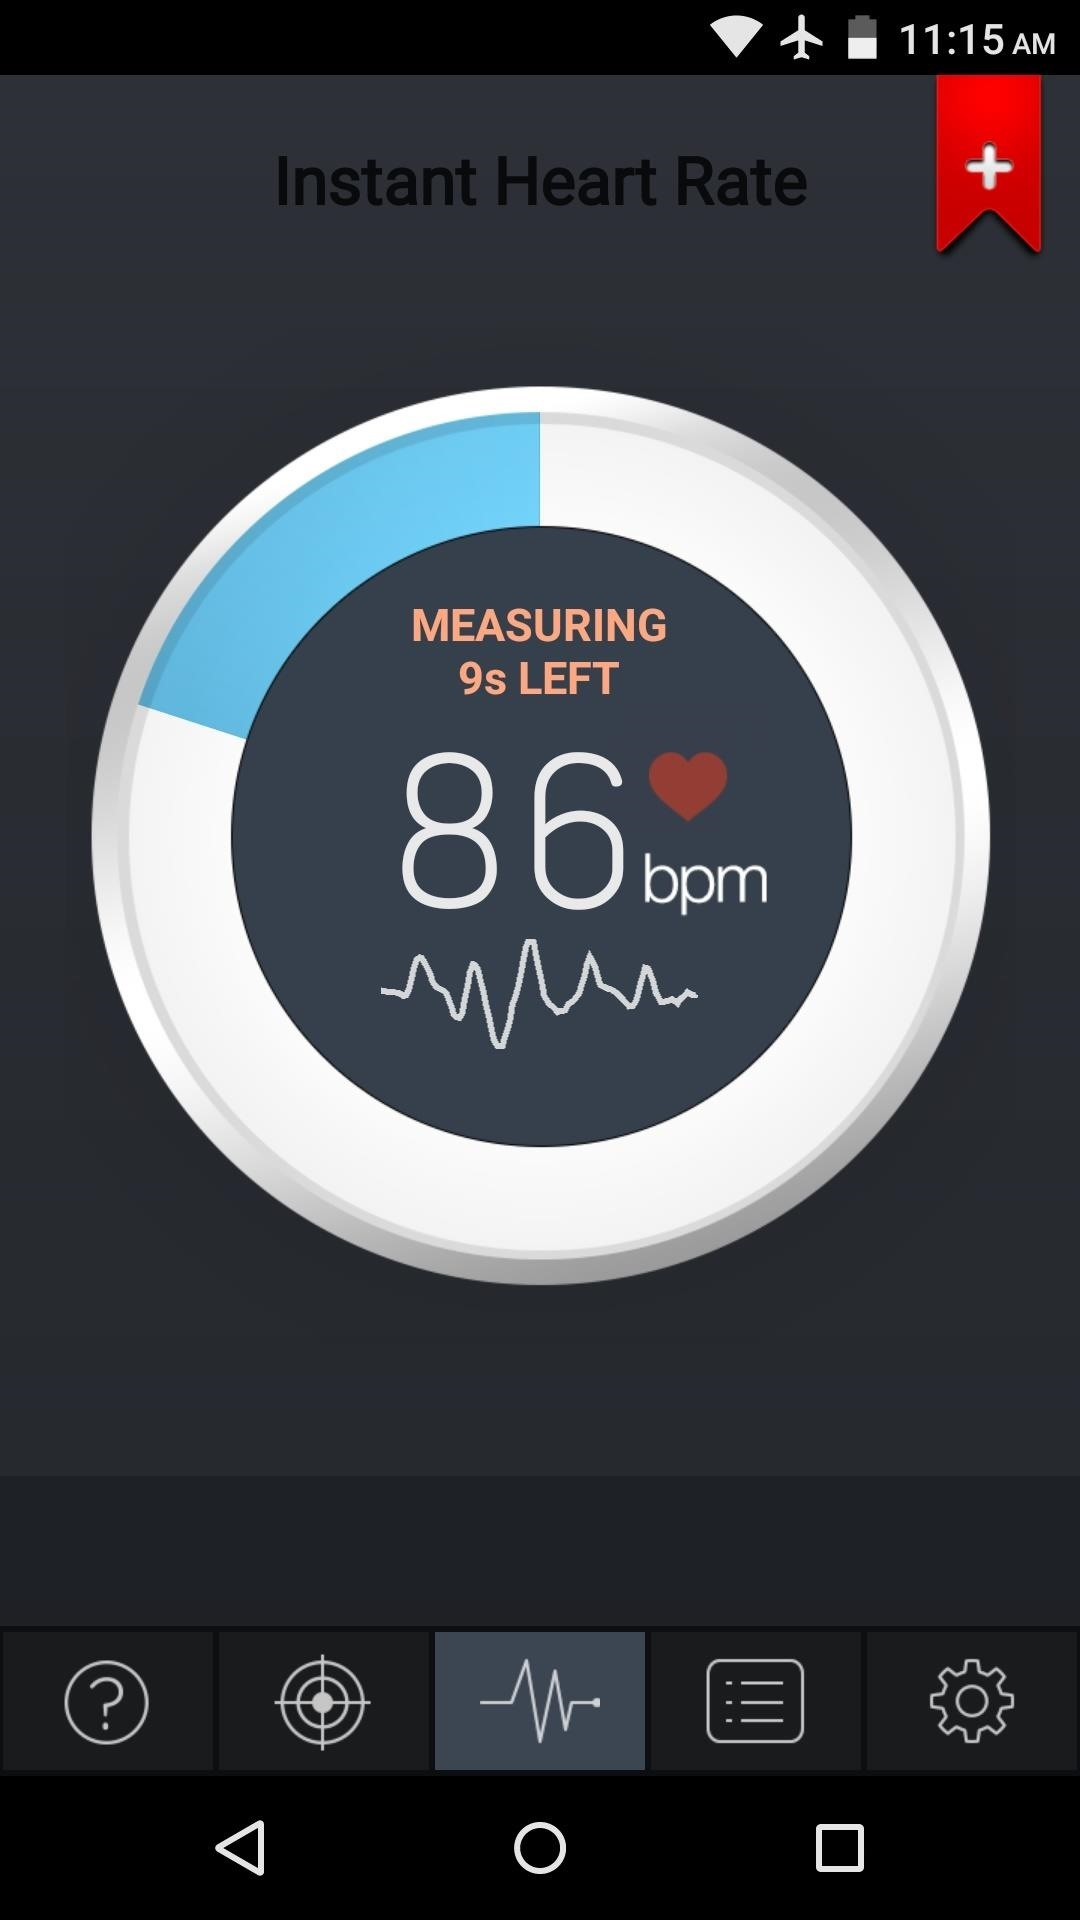
\includegraphics[scale=0.05]{images/heart_app1.jpg}
	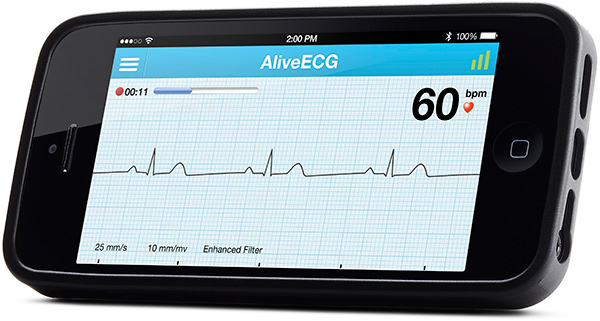
\includegraphics[scale=0.2]{images/heart_app2.jpg}
    \caption{a. Jam produksi fitbit; b. Finger clip PPG; c. Portable ECG; d. Heart Rate App; e. Heart Rate App 2}
\end{figure}

\section{Node.Js, Mongo.Db dan Express.Js}
Sebuah sistem monitoring yang dapat berjalan secara Ubiquitous haruslah dibangun dengan konsep \textit{Internet of Things} (IoT). IoT ialah konsep dimana objek objek (Things) dapat saling berinteraksi pada jaringan Internet tanpa membutuhkan manusia. Pada konsep IoT diperlukan setidaknya 3 komponen yaitu Sensor, Server dan Actuator. Sensor berfungsi sebagai pengambil data. Server berfungsi sebagai pengolah data yang menjalankan \textit{web service} (layanan web). Actuator berfungsi sebagai pelaksana keputusan, seperti mengeluarkan suara dan membelokkan/memutus arus listrik.

Node.Js, Mongo.Db dan Express.Js, sesuai urutan, merupakan teknologi Javascript (JS) \textit{runtime}, \textit{Document Db  (database)}, dan \textit{Web Framework} berbasis JS. Ketiga hal ini dibutuhkan untuk membangun sebuah web service. Node.Js dirancang menggunakan skema \textit{event-driven} dan \textit{non-blocking IO}, sangat sesuai untuk aplikasi \textit{data-intensive real-time} \cite{nodejs}. Node.JS juga telah terbukti secara performansi lebih cepat dari bahasa scripting lain seperti PHP, Python, dan Ruby bahkan tidak jauh lambat dibanding bahasa ter-\textit{compile} seperti JAVA, C, dan C++ \cite{node_comparisson}.

\begin{figure}[H]
    \centering
	
\includegraphics[scale=0.15]{images/nodejs.png}
    
\includegraphics[scale=0.3]{images/mongodb.png}
	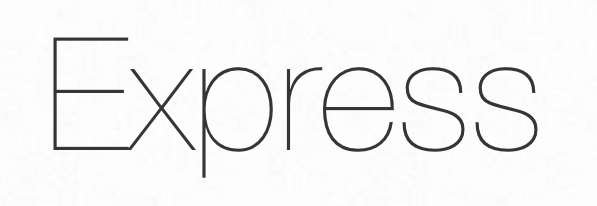
\includegraphics[scale=0.2]{images/express.png}
    \caption{a. Node JS; b. Mongo DB; c. Express}
\end{figure}

\section{ESP-12}
ESP-12 adalah salah satu tipe \textit{System on Module} (SoC) yang diproduksi oleh Espressif dari China. SoC berarti papan sirkuit yang telah terintegrasi oleh sistem tertentu. Kelebihan utama ESP ialah ukurannya yang kecil (16x24x3 mm) tapi dapat berfungsi sebagai controller dan telah dilengkapi modul Wi-Fi. Hal ini memungkinkan komunikasi sensor-server melalui jaringan WiFi tanpa perlu menambah modul jaringan lagi.

\begin{figure}[H]
	\centering
	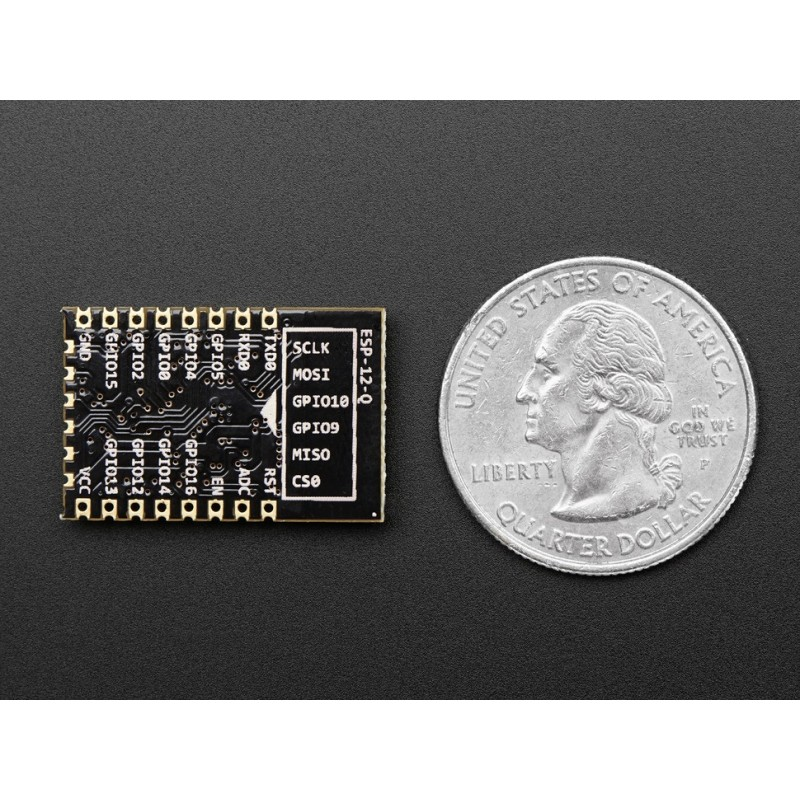
\includegraphics[scale=0.22]{images/esp12e.jpg}
	\caption{ESP-12E dengan koin 1/4 dollar amerika}
\end{figure}

\section{Protokol MQTT}
Message Queuing Telemetry Transport (MQTT) adalah protokol transport
dengan skema komunikasi publish dan subscribe. MQTT dirancang menjadi protokol yang ringan, terbuka dan sederhana. Karakteristik ini membuat MQTT sangat tepat untuk digunakan sebagai protokol komunikasi machine-to-machine (M2M) dan Internet of Things (IoT). Protokol ini menggunakan TCP/IP pada layer transport. Terdapat tiga level Qualities of Service (QoS) dalam penyampaian pesan yaitu:
\begin{enumerate}
	\item QOS 0 atau “At most once”, dimana pesan dikirim dengan skema \textit{fire-and-forget} yang berarti tidak ada upaya menjamin pesan yang dikirim dapat sampai ke tujuan.
	\item QOS 1 atau “At least once”, dimana pesan dikirim dengan jaminan setidaknya pesan sampai sekali ke tujuan. Sehingga memungkinkan terjadinya duplikasi pesan di tujuan akibat pesan yang dikirim ulang dari pengirim.
	\item QOS 2 atau "Exactly once", dimana pesan dikirm dengan jaminan diterima tepat sekali ke tujuan. Sehingga tidak ada pesan yang terduplikasi di tujuan.	
\end{enumerate}

\begin{figure}[H]
	\centering
	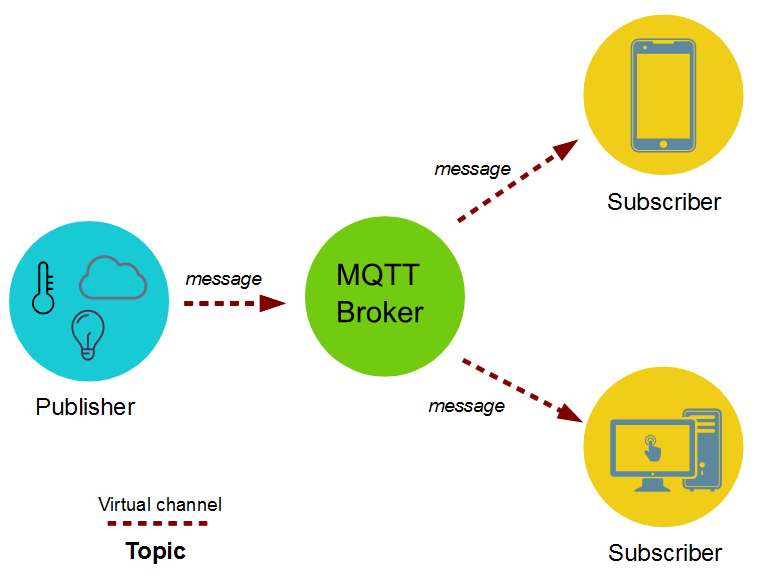
\includegraphics[scale=0.45]{images/mqtt.png}
	\caption{Cara kerja MQTT}
\end{figure}

